%\section{Стабилизация неустойчивых стационарных решений уравнения Бюргерса}
%\vspace{1em}
\chapter{Стабилизация неустойчивых стационарных решений уравнения Бюргерса}


\section{Постановка задачи}
\vspace{1em}

Рассмотрим уравнение Бюргерса с вязкостью $\nu > 0$ на интервале $\Omega$

\begin{equation}\label{burger}
    u_t - \nu u_{xx} + u_x u = f + y, \ u|_{\Gamma} = u_b, \quad t > 0.
\end{equation}

Функция $f = f(x)$, $x \in \Omega$ является заданной, а функция $y = y(x, u)$
рассматривается как управление, носитель которого при фиксированном $t > 0$
содержиться в $\bar{\omega}$, где $\bar{\omega}$ - заданная подобласть $\Omega$.
Через $\Gamma = \{0, 1\}$ обозначена граница $\Omega$, $u_b \in \mathbb{R}^2$\\

Пусть $U$ - стационарное решение \eqref{burger}, то есть

\begin{equation}\label{stationary_sol}
    -\nu U_{xx} + U U_x = f, \ U|_{\Gamma} = u_b,
\end{equation}
и функция $U$ является неустойчивой особой точкой динамической системы, порождаемой
эволюционным уравнение \eqref{burger} в фазовом пространстве $H$.
Задача стабилизации состоит в следующем:\\

\textit{Для заданного} $\sigma > 0$ 
\textit{требуется найти оператор управления с обратной связью} 
$y = \Lambda(u - U) : H \to H$ \textit{такой, что} $\mathbf{supp} \ y (\cdot,t) \subset 
\bar{\omega}$ \textit{и решение замкнутой системы}

\begin{equation}
    u_t - \nu u_xx + u u_xx = f + \Lambda(u - U), \ u|_{\Gamma} = u_b,
    \ t > 0, \quad u|_{t=0} = u_0
\end{equation}
\textit{сходилось к} $U$ \textit{с заданной скоростью} $\sigma$

\begin{equation}
    \norm{u(t) - U}_{L^2(\Omega)} \le C e^{-\sigma t} \ \text{при } t
    \to +\infty,
\end{equation}
\textit{если величина} $\norm{u_0 - U}_{L^2(\Omega)}$ \textit{достаточно мала}\\

Пусть $\varphi = u - U$, тогда

\begin{gather}\label{fluct}
    \varphi_t - \nu \varphi_{xx} + \varphi U_x + (\varphi + U)\varphi_x =
    \Lambda(\varphi),\\* 
    \varphi|_{\Gamma} = 0, \ t > 0,\\*
    \varphi|_{t = 0} = \varphi_0 = u_0 - U.
\end{gather}

Требуется чтобы $\norm{\varphi(t)}_{L^2(\Omega)} \le C e^{-\sigma t}$ при $t \to
+\infty$, если мала норма $\norm{\varphi_0}_{L^2(\Omega)}$

\section{Неустойчивость стационарных решений shock-like}
\vspace{1em}

Рассмотрим семейство стационарных решений типа shock-like \cite{KMV}

\begin{equation}\label{shock_like}
    U(x) = -2\tau\tanh{(\tau(x - \frac{1}{2}))}, \ \text{где } \tau \ge 0.
\end{equation}

\begin{figure}
    \centering
    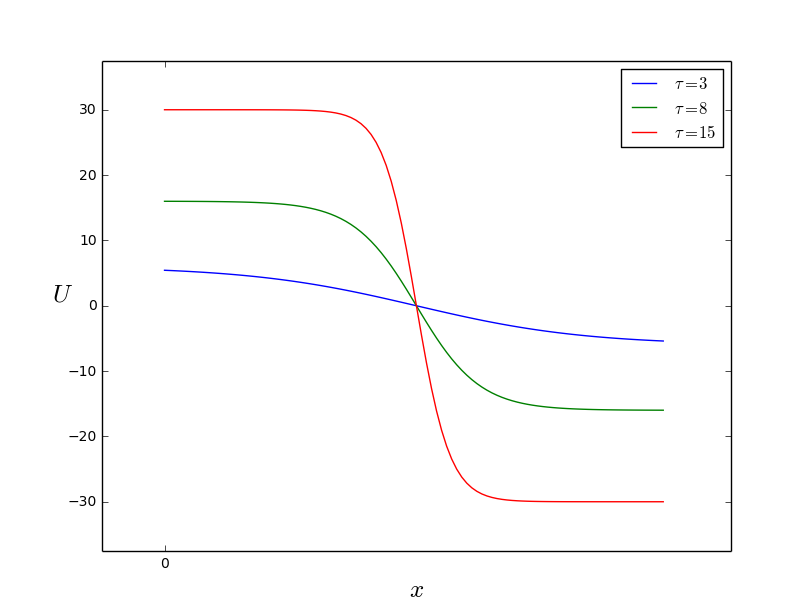
\includegraphics[width=4in]{fig1}
    \caption{$U(x)$ при разных $\tau$}
\end{figure}

Для изучения устойчивости системы \eqref{fluct} без стабилизирующего управления, 
мы линеаризуем её

\begin{gather}\label{linearized}
    \theta_t = \theta_{xx} + 2 \tau (\tanh(\tau(x - \frac{1}{2}))\theta)_x, \\*
    \theta(0, t) = \theta(1, t) = 0,
\end{gather}
где $\theta(x, t)$ - решение уравнения \eqref{linearized}, которое является
линеаризацией \eqref{fluct}. Заметим что \eqref{linearized} является  уравнение 
конвенкции-диффузии-реакции. Для простоты изучения устойчивости, мы избавимся 
от конвекционого члена используя преобразование 
$\zeta(x, t) = G(x)\theta(x, t)$, где 

\begin{equation}
    G(x) = \frac{\cosh(\tau(x - \frac{1}{2}))}{\cosh(\frac{\tau}{2})}.
\end{equation} 

Имеем 

\begin{gather} \label{transf_linear}
    \zeta_t = \zeta_{xx} + \tau^2 \left( \frac{2}{\cosh^2(\tau(x -
    \frac{1}{2}))} - 1 \right) \zeta, \\* 
    \zeta(0) = \zeta(1) = 0.
\end{gather}
Для $\tau = 0$ система нейтрально устойчива. Для $\tau > 0$, коэффициент 
$\mu = \left(\frac{2}{\cosh^2(\tau(x - \frac{1}{2}))} - 1 \right)$  в 
\eqref{transf_linear} является "неустойчивым" в окрестности 
$x = \frac{1}{2}$ (Рис 2.), т.е. положительность этого члена ведет к
неустойчивости системы.


\begin{figure}
    \centering
    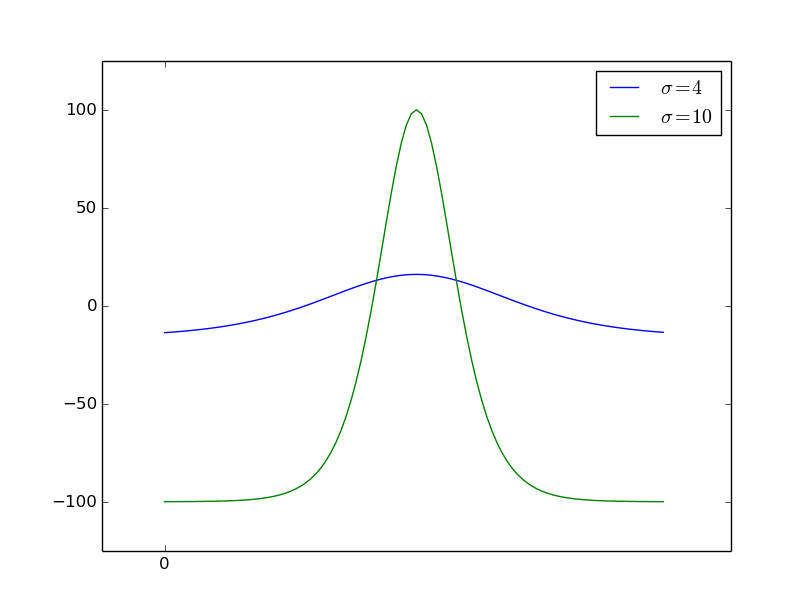
\includegraphics[width=4in]{fig2}
    \caption{График $\mu$ в \eqref{transf_linear}}
\end{figure}
